\chapter{Resultados e discussão}\label{resultados-e-discussao}
\section{Protocolo de comparação e proveniência}
Os resultados apresentados neste capítulo correspondem a duas execuções retrospectivas consolidadas sobre a mesma base histórica: a inferência fora do período de ajuste (\texttt{OOT\_MULTIVIEW}, ajustada nos cortes de 31/08, 30/09 e 31/10/2026 com 189.341 amostras elegíveis e avaliada em 19/11/2026) e o monitoramento diário calibrado por regras (\texttt{DAILY\_RULES}, cobrindo 19 cortes diários entre 1\textordmasculine{} e 19/11/2026). As execuções foram versionadas. Na inferência OOT, os parâmetros de pré-processamento, os quantis de normalização e o limiar de decisão foram congelados no conjunto de ajuste. O índice \texttt{experiments/runs/latest\_suite.json} identifica as execuções. Os manifestos registram versão do código e configuração. Os hashes SHA-256 das tabelas de decisões OOT e diária coincidem com o registro de auditoria de 25/11. A conferência nominal das decisões depende de acesso autorizado aos registros por UC; as figuras do artigo apresentam dados agregados ou mascarados. O funil sequencial e a ablação interna dos detectores possuem critérios próprios, descrevendo a composição da lista e a estabilidade dos escores.
\section{Inferência multivisão fora do período de ajuste}
Em 19 de novembro de 2026, avaliaram-se 65.686 UCs na execução consolidada pós-saneamento (\texttt{20261125\_134559\_972\_oot\_multiview}, código base \texttt{c1539b4}). A política de qualidade classificou 62.857 como elegíveis (95,69\%) e 2.829 em quarentena (4,31\%). O escore médio populacional foi 0,2865 e o percentil 95 atingiu 0,9438. A política multivisão selecionou 6.037 candidatos. Na coorte avaliada, a indicação de vistoria coincidiu com a flag de anomalia elétrica nas 65.686 linhas. O limiar congelado do escore elétrico foi $\tau_{train}=0{,}5131$; a qualidade da telemetria e as regras diagnósticas orientaram a interpretação das evidências. O Isolation Forest (IF) de referência, com limiar congelado de 0,643, selecionou 3.122. A diferença de contagens mede seletividade sob políticas distintas.

A Tabela \ref{classes} discrimina os destinos diagnósticos exclusivos atribuídos às 65.686 unidades na execução de 25/11. A soma das três categorias de caráter elétrico ou metrológico (anomalia elétrica, possível geração distribuída e falha metrológica: $4.087 + 1.451 + 515 = 6.053$ UCs) difere em 16 unidades dos 6.037 candidatos selecionados. A categorização diagnóstica cobre toda a coorte, enquanto a fila aplica critérios próprios de elegibilidade e materialidade. O cruzamento das decisões por UC identificou as 16 exclusões na categoria de possível GD: 1.435 das 1.451 unidades dessa categoria entraram na fila. As 16 restantes apresentavam confiabilidade elétrica (\texttt{is\_reliable\_elec=True}) e não estavam sinalizadas como anomalia elétrica (\texttt{is\_elec\_anomaly=False}). Essa coincidência observada entre flags é específica da campanha, não uma equivalência universal entre categoria e decisão. Já as 12.084 UCs classificadas em mudança de classe comportamental decorrem de transições de rótulo entre arquétipos de carga na janela comparada, não constituindo escore calibrado de anomalia nem integrando automaticamente a carteira de 6.037 candidatos.

\begin{table}[htbp]\centering\small\caption{Distribuição das hipóteses diagnósticas no OOT de 19 de novembro}\label{classes}
\begin{tabular}{>{\raggedright\arraybackslash}p{\dimexpr 0.8\linewidth-2\tabcolsep\relax}>{\raggedright\arraybackslash}p{\dimexpr 0.2\linewidth-2\tabcolsep\relax}}\toprule
Hipótese ou estado analítico & UCs \\ \midrule
Operação regular segundo os critérios da política & 44.674 \\
Mudança de classe comportamental & 12.084 \\
Anomalia elétrica compatível com hipótese de PNT & 4.087 \\
Gargalo coletivo da rede de comunicação por rádio & 1.829 \\
Possível geração distribuída sem correspondência cadastral & 1.451 \\
Anomalia isolada de comunicação & 910 \\
Hipótese de falha metrológica com registrador travado & 515 \\
Início de perfil de nova UC & 71 \\
Transição associada à troca de medidor & 65 \\
Total & 65.686 \\
\bottomrule\end{tabular}
\par\small Fonte: elaboração própria a partir da execução \texttt{20261125\_134559\_972\_oot\_multiview}.
\end{table}
\section{Série diária calibrada e dinâmica das listas}
A série DAILY\_RULES acumulou 1.248.501 janelas UC \ensuremath{\times} corte entre 1\textordmasculine{} e 19 de novembro. A média foi de 5.387,7 candidatos por dia. A lista passou por um máximo de 6.728 em 2 de novembro e um mínimo de 4.737 em 15 de novembro. No último corte, 4.978 UCs integraram a lista, das quais 4.342 permaneceram em relação à véspera e 636 ingressaram. Outras 588 saíram da lista do dia anterior. Assim, a variação líquida de 48 UCs reconciliou a passagem de 4.930 para 4.978.

\begin{figure}[htbp]\centering\caption{Candidatos e transições da lista diária sob a regra calibrada, de 1\textordmasculine{} a 19 de novembro}\label{diaria}
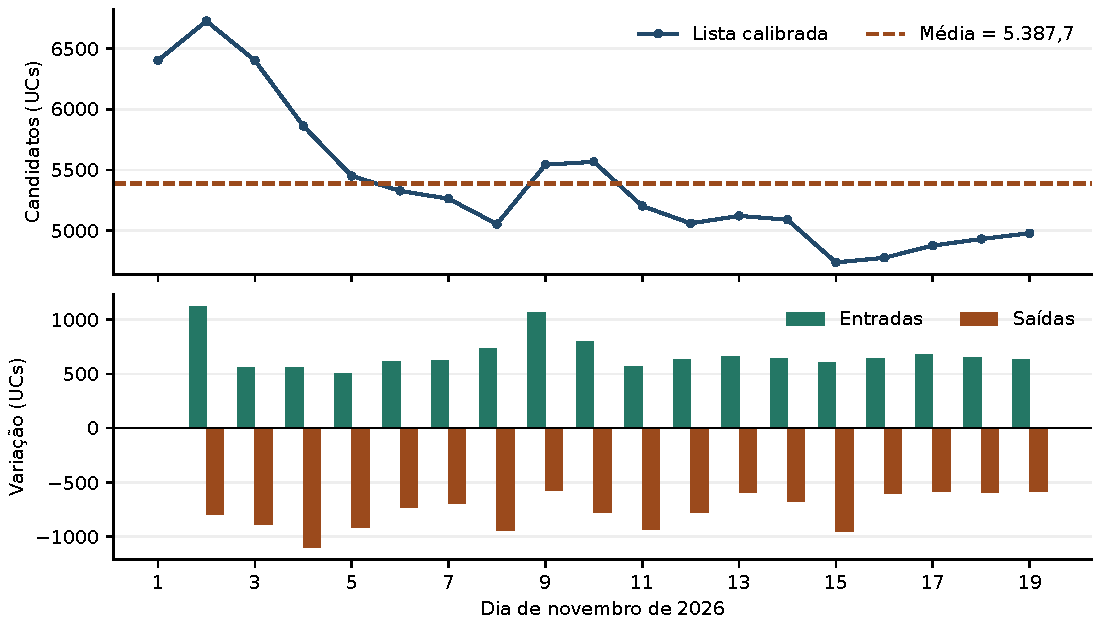
\includegraphics[width=0.96\textwidth,height=0.46\textheight,keepaspectratio]{figuras/diaria.pdf}
\par\small Fonte: elaboração própria com base nos 19 cortes diários calibrados.
\end{figure}
Na Figura \ref{diaria}, o primeiro ponto estabeleceu o estoque inicial de 6.404 candidatos. As barras de movimento começam no segundo dia, primeira data com comparação entre dois cortes observados. A saída da lista representa perda de pertinência ao critério do dia. A inferência OOT produziu 6.037 candidatos na mesma data final sob ajuste e política próprios. A diferença líquida de 1.059 entre as listas (6.037 vs. 4.978) não identifica quais UCs trocaram de prioridade. A série legada, próxima de 30 mil candidatos, empregava uma regra de desequilíbrio de corrente sem restrição de materialidade e não corresponde à política calibrada da Figura \ref{diaria}. De 2 a 6 de novembro, a lista calibrada passou de 6.728 para 5.327; em 6/11, as 612 entradas e 735 saídas produziram saldo de $-123$. O movimento descreve a pertinência à regra diária, sem estabelecer a causa física de cada transição. O cruzamento por UC em 19/11 identificou 2.069 unidades comuns, 3.968 exclusivas do OOT e 2.909 exclusivas da regra diária.

\section{Sensibilidade da cobertura, ablação e composição do Top-K}
No ensaio de sensibilidade (\texttt{20261125\_134940\_636\_gating\_sensitivity}), manteve-se a coorte de 65.686 UCs e variou-se o limiar de cobertura entre 50\% e 90\%. A Tabela \ref{gating} apresenta a população elegível e a divisão dos candidatos elétricos do ensaio entre retenção e quarentena. A elevação de 70\% para 90\% reduziu os elegíveis de 62.857 para 59.091 e alterou a composição da lista. As contagens de sinalizações brutas variaram entre linhas. O desenho mede a resposta da política avaliada em cada limiar, e não apenas a aplicação de uma máscara sobre escores fixos. Os candidatos interceptados não constituem falsos negativos confirmados.

\begin{table}[htbp]\centering\small\caption{Sensibilidade à cobertura no corte de 19 de novembro}\label{gating}
\begin{tabular}{>{\raggedright\arraybackslash}p{\dimexpr 0.13\linewidth-2\tabcolsep\relax}>{\raggedright\arraybackslash}p{\dimexpr 0.17\linewidth-2\tabcolsep\relax}>{\raggedright\arraybackslash}p{\dimexpr 0.18\linewidth-2\tabcolsep\relax}>{\raggedright\arraybackslash}p{\dimexpr 0.16\linewidth-2\tabcolsep\relax}>{\raggedright\arraybackslash}p{\dimexpr 0.16\linewidth-2\tabcolsep\relax}>{\raggedright\arraybackslash}p{\dimexpr 0.2\linewidth-2\tabcolsep\relax}}\toprule
Limiar & Elegíveis & Quarentena & Brutos & Retidos & Interceptados \\ \midrule
50\% & 63.371 & 2.315 & 6.729 & 5.945 & 784 \\
60\% & 63.111 & 2.575 & 6.700 & 5.793 & 907 \\
70\% & 62.857 & 2.829 & 6.767 & 5.788 & 979 \\
80\% & 61.530 & 4.156 & 6.904 & 5.728 & 1.176 \\
90\% & 59.091 & 6.595 & 7.398 & 5.531 & 1.867 \\
\bottomrule\end{tabular}
\par\small Fonte: elaboração própria a partir da execução \texttt{20261125\_134940\_636\_gating\_sensitivity}.
\end{table}
A 70\%, o ensaio de cobertura reteve 5.788 candidatos elétricos e interceptou 979 na quarentena técnica, frente a 6.037 candidatos no OOT completo (diferença líquida de 249 unidades). Na sensibilidade, o detector é reajustado nas UCs elegíveis do próprio corte e aplica o limiar fixo de 0,5226, conforme a configuração histórica da execução de 25/11 (código base \texttt{c1539b4}; Apêndice~\ref{ap:proveniencia}). A variante posterior que recalcula o limiar a cada reajuste não foi utilizada para os números desta tabela. No OOT, o ajuste precede o corte e o limiar congelado é 0,5131. A diferença líquida entre as contagens não identifica 249 inclusões individuais. Na comparação da ordenação com a referência sem filtro, a correlação de Spearman a 70\% foi 0,9952, com Jaccard de 0,7900 no Top-5\%. A concordância global elevada permitiu mudanças relevantes na extremidade de interesse.

\begin{figure}[htbp]\centering\caption{Resposta ao limiar de cobertura e funil sequencial no corte OOT}\label{funil}
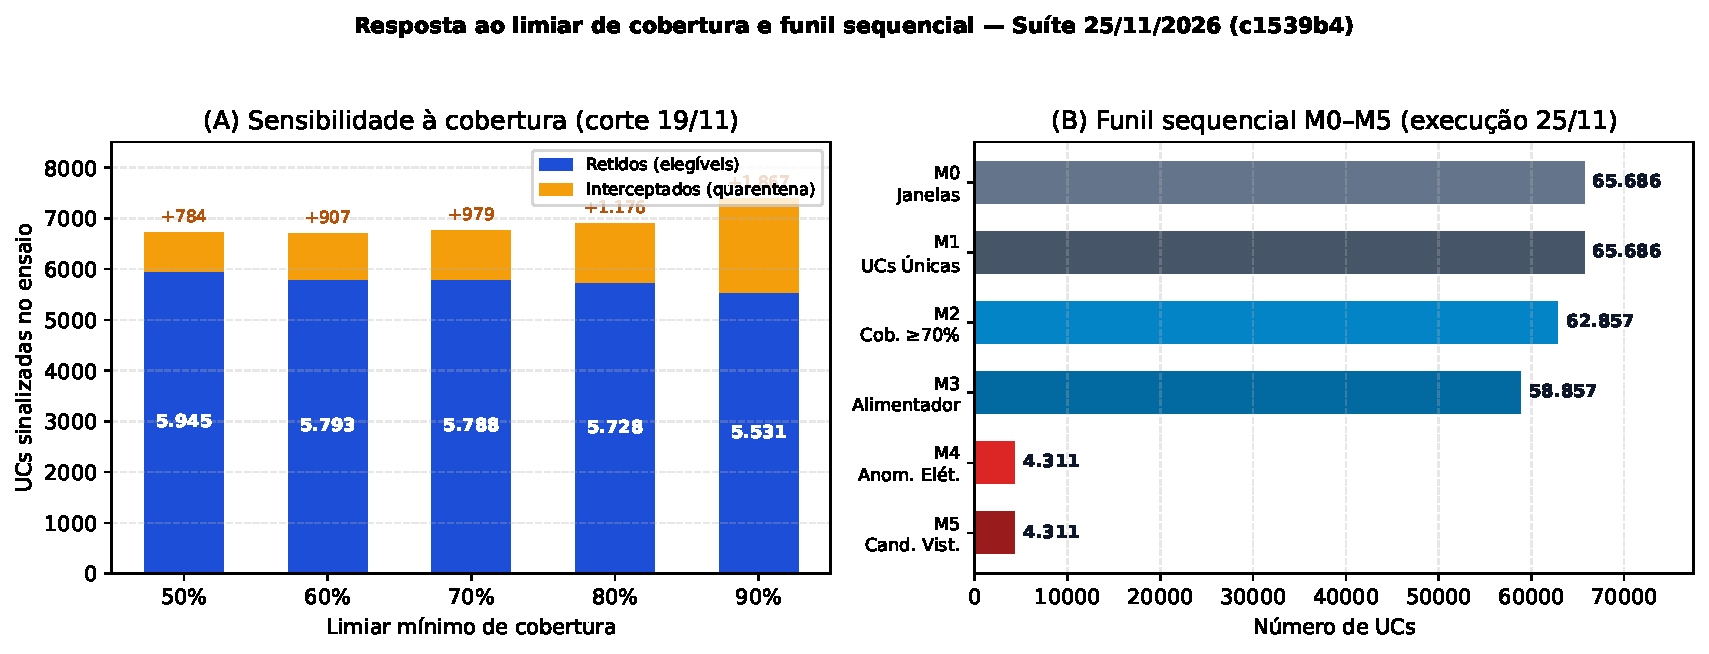
\includegraphics[width=0.96\textwidth,height=0.46\textheight,keepaspectratio]{figuras/funil.pdf}
\par\small Fonte: elaboração própria com base nos ensaios de cobertura e ablação de novembro.
\end{figure}
A Figura \ref{funil} apresenta as duas experiências no mesmo corte. No funil corrigido (\texttt{20261125\_134849\_083\_ablation\_m0\_m5}), M0 e M1 reuniram as mesmas 65.686 UCs, pois a coorte continha uma observação por unidade. M2 manteve 62.857 com cobertura adequada. M3 exigiu alimentador e preservou 58.857. M4 reteve 4.311 por critérios estatísticos e elétricos e M5 manteve as mesmas 4.311 após o filtro operacional. Os estágios formam conjuntos aninhados que admitem igualdade. A igualdade M4 = M5 caracteriza apenas o corte analisado e não demonstra redundância geral da etapa M5. As 1.726 UCs que completam a diferença para os 6.037 candidatos gerais não possuíam alimentador cadastrado para a análise contextual.

No ensaio interno, fixou-se um orçamento de 2.000 posições. O índice de Jaccard entre duas listas é a cardinalidade da interseção dividida pela da união. Na Tabela \ref{ablacao}, na execução corrigida, 1.813 UCs comuns em duas listas de 2.000 (sem LOF) implicaram união de 2.187 e índice de 0,8290 (187 substituições). Sem PCA, ocorreram 166 substituições (Jaccard = 0,8467); e no núcleo de quatro detectores, 254 substituições (Jaccard = 0,7746).

\begin{table}[htbp]\centering\small\caption{Sensibilidade do ranking à retirada de detectores (execução corrigida)}\label{ablacao}
\begin{tabular}{>{\raggedright\arraybackslash}p{\dimexpr 0.22\linewidth-2\tabcolsep\relax}>{\raggedright\arraybackslash}p{\dimexpr 0.14\linewidth-2\tabcolsep\relax}>{\raggedright\arraybackslash}p{\dimexpr 0.16\linewidth-2\tabcolsep\relax}>{\raggedright\arraybackslash}p{\dimexpr 0.16\linewidth-2\tabcolsep\relax}>{\raggedright\arraybackslash}p{\dimexpr 0.15\linewidth-2\tabcolsep\relax}>{\raggedright\arraybackslash}p{\dimexpr 0.17\linewidth-2\tabcolsep\relax}}\toprule
Variante & Spearman & Jaccard Top-5\% & Comuns & Trocas & Jaccard Top-2.000 \\ \midrule
Comitê completo & 1,0000 & 1,0000 & 2.000 & 0 & 1,0000 \\
Sem LOF & 0,9872 & 0,8283 & 1.813 & 187 & 0,8290 \\
Sem PCA & 0,9983 & 0,8764 & 1.834 & 166 & 0,8467 \\
Núcleo de quatro & 0,9841 & 0,7721 & 1.746 & 254 & 0,7746 \\
\bottomrule\end{tabular}
\par\small Fonte: elaboração própria a partir da execução \texttt{20261125\_134849\_083\_ablation\_m0\_m5}.
\end{table}
\section{Correlação, empates e estabilidade das escalas}
A Figura~\ref{correlacao} compara a ordenação dos seis detectores e do consenso elétrico na mesma execução OOT. A correlação de Spearman foi calculada sobre os postos das 65.686 UCs, atribuindo posto médio aos empates. A concordância descreve a semelhança entre ordenações. A matriz não compara populações históricas distintas nem permite atribuir isoladamente diferenças de correlação às correções do LOF e da PCA. Na campanha histórica, os escores LOF apresentaram mediana e percentis 95 e 99 iguais a zero na precisão de quatro casas decimais. Uma hipótese é a compressão da escala causada por empates e valores extremos; a transformação logarítmica e o tratamento de quantis degenerados procuram limitar esse efeito. O resíduo da PCA, por sua vez, mede afastamento do subespaço linear, não apenas extremidade marginal, de modo que sua discordância com os demais detectores não implica inversão de sinal. A padronização interna reduz a influência de diferenças de escala. Essas explicações motivam a auditoria, mas não isolam o efeito causal de cada correção. Sua relação com o acerto em campo depende de inspeções com desfecho conhecido.

\begin{figure}[htbp]\centering\caption{Correlação de postos entre detectores e consenso elétrico no OOT}\label{correlacao}
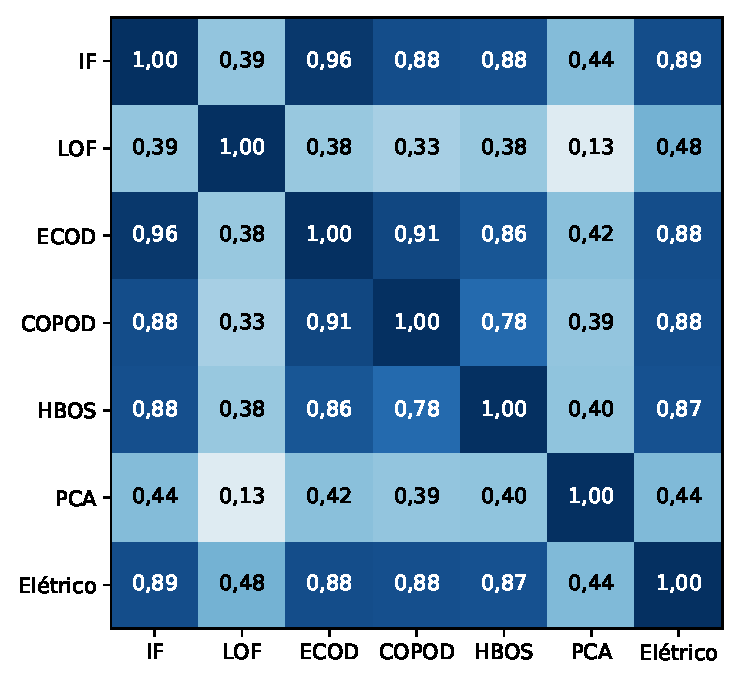
\includegraphics[width=.82\linewidth]{figuras/correlacao.pdf}
\par\small Fonte: elaboração própria a partir dos escores individuais da inferência de 19/11.
\end{figure}
Na experiência de estabilidade sobre 65.686 UCs (\texttt{20261125\_135109\_678\_}\allowbreak\texttt{score\_stability}), a retirada do 1\% extremo deixou 65.029 observações. A normalização pelos extremos de cada lote (\texttt{batch\_minmax}) produziu deslocamento médio absoluto de 0,034047 e máximo de 0,2291. Com os quantis de referência congelados (\texttt{frozen\_quantile} e \texttt{frozen\_ecdf}), ambos foram zero nessa perturbação. Na auditoria individual de detectores sobre as 65.686 UCs da coorte OOT (\texttt{detector\_individual\_audit.csv}), as correlações de Spearman frente ao consenso foram 0,8858 (IF), 0,4763 (LOF), 0,8829 (ECOD), 0,8755 (COPOD), 0,8738 (HBOS) e 0,4396 (PCA). O ensaio de estabilidade demonstrou invariância à composição do lote sob a perturbação testada. As correlações descrevem a configuração OOT final; não isolam causalmente o efeito das correções de escala.

\section{Estudos de caso e anatomia da detecção}\label{estudos-caso-reconciliados}
O exame longitudinal integra grandezas elétricas, cobertura, vínculo histórico e hipótese diagnóstica. Os casos a seguir, reproduzidos sobre os registros de origem da suíte de 25/11 (\texttt{20261125\_135558\_880\_case\_traces}), ilustram o exame das evidências de mudança e a reconciliação formal das inconsistências de qualidade.

Na UC \texttt{908***00} (\texttt{NIO-435***63}), o cadastro registrou atualização administrativa em 31 de outubro (\texttt{DATA\_INSTALACAO}), embora as medições anteriores permanecessem vinculadas ao mesmo NIO. Houve intervalo de indisponibilidade de dois dias e mudança persistente por 20 dias até 19/11. A FA passou de 18,05 para 5,72 kWh/dia, queda aproximada de 68,3\%. Registrou-se RA em 12 dias posteriores, com valores diários de até 31,27 kWh/dia (razão reversa máxima de 0,5069). O escore elétrico consolidado atingiu 1,0000 na execução de 25/11. A Figura \ref{fig:caso-908xxx00-completo} apresenta a energia diária FA/RA e a cobertura ajustada à cadência de 10~min.

\begin{figure}[htbp]\centering\caption{Série temporal completa observada para a UC \texttt{908***00} (02/08 a 19/11/2026, medidor \texttt{NIO-435***63}): (A) energia ativa direta FA e reversa RA diárias; (B) cobertura ajustada à cadência de 10~min}\label{fig:caso-908xxx00-completo}
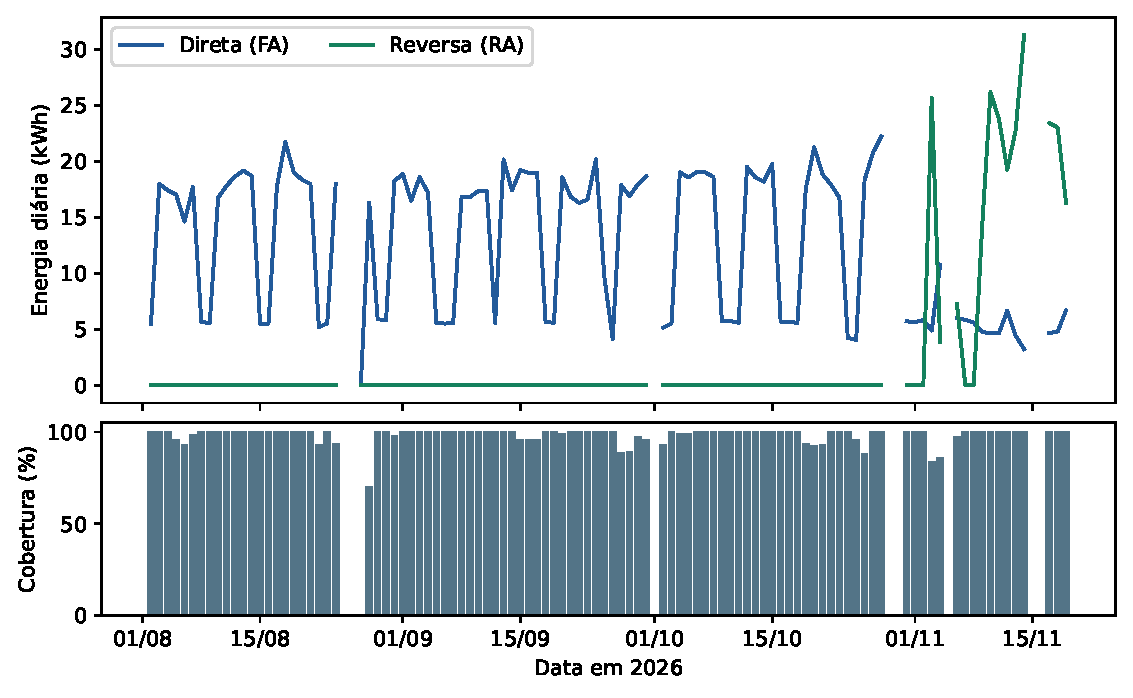
\includegraphics[width=0.96\textwidth,height=0.46\textheight,keepaspectratio]{figuras/fig_caso_908xxx00_fa_ra_completo.pdf}
\par\small Fonte: elaboração própria a partir dos registros longitudinais da UC.
\end{figure}
A continuidade do NIO é compatível com a preservação do histórico do mesmo equipamento, sem sustentar, isoladamente, ausência de intervenção física. A combinação de mudança de patamar e fluxo reverso sustentou a hipótese diagnóstica de possível GD não cadastrada a confrontar com o cadastro em inspeção futura.

Na UC \texttt{291***96} (\texttt{NIO-423***54}), os registros de origem em \texttt{ami\_interval} confirmam cadência nativa de 10 minutos (6 leituras/h; 144 registros/dia); em \texttt{ami\_registers}, foram observadas 314 leituras do registrador acumulado \texttt{RA\_TOTAL} ($764{,}601 \to 2.967{,}725$~kWh) até 05/11/2026, com incremento de 2.203,124 kWh entre 01/08 às 00h e 05/11 às 18h UTC (96,75 dias decorridos, média de 22,77 kWh/dia), mesmo com \texttt{DATA\_REMOCAO = 2026-06-11} no cadastro CIS. Entre 06 e 19/11/2026, ocorreu silêncio completo de transmissão, o que explica a cadência pontual ausente (\texttt{None}) e o indicador de qualidade OOT reportado como 3,33\% (1 dia confiável em 30, proporção distinta da completude intervalar) no corte de 19/11, mantendo a unidade em quarentena técnica de comunicação (\texttt{ANOMALIA\_COMUNICACAO\_ISOLADA}), sem inclusão na fila de candidatos comerciais dessa política (Figura \ref{fig:caso-291xxx96-registradores}). A progressão do registrador reverso após a retirada declarada justifica auditar a ordem de remoção, a eventual reinstalação e o vínculo comercial vigente no período. A quarentena orienta o reparo de comunicação e preserva essa pendência cadastral. Os registros isolados não estabelecem a identidade do ponto de injeção após a retirada nem irregularidade de faturamento.

\begin{figure}[htbp]\centering\caption{Auditoria longitudinal da UC \texttt{291***96} (\texttt{NIO-423***54}, 01/08 a 19/11/2026): (A) evolução acumulada de 314 leituras do registrador \texttt{RA\_TOTAL}, delta diário e hiatos de comunicação; (B) horários empíricos de leitura intervalar (10~min) e de registradores (00h/06h/12h/18h UTC)}\label{fig:caso-291xxx96-registradores}
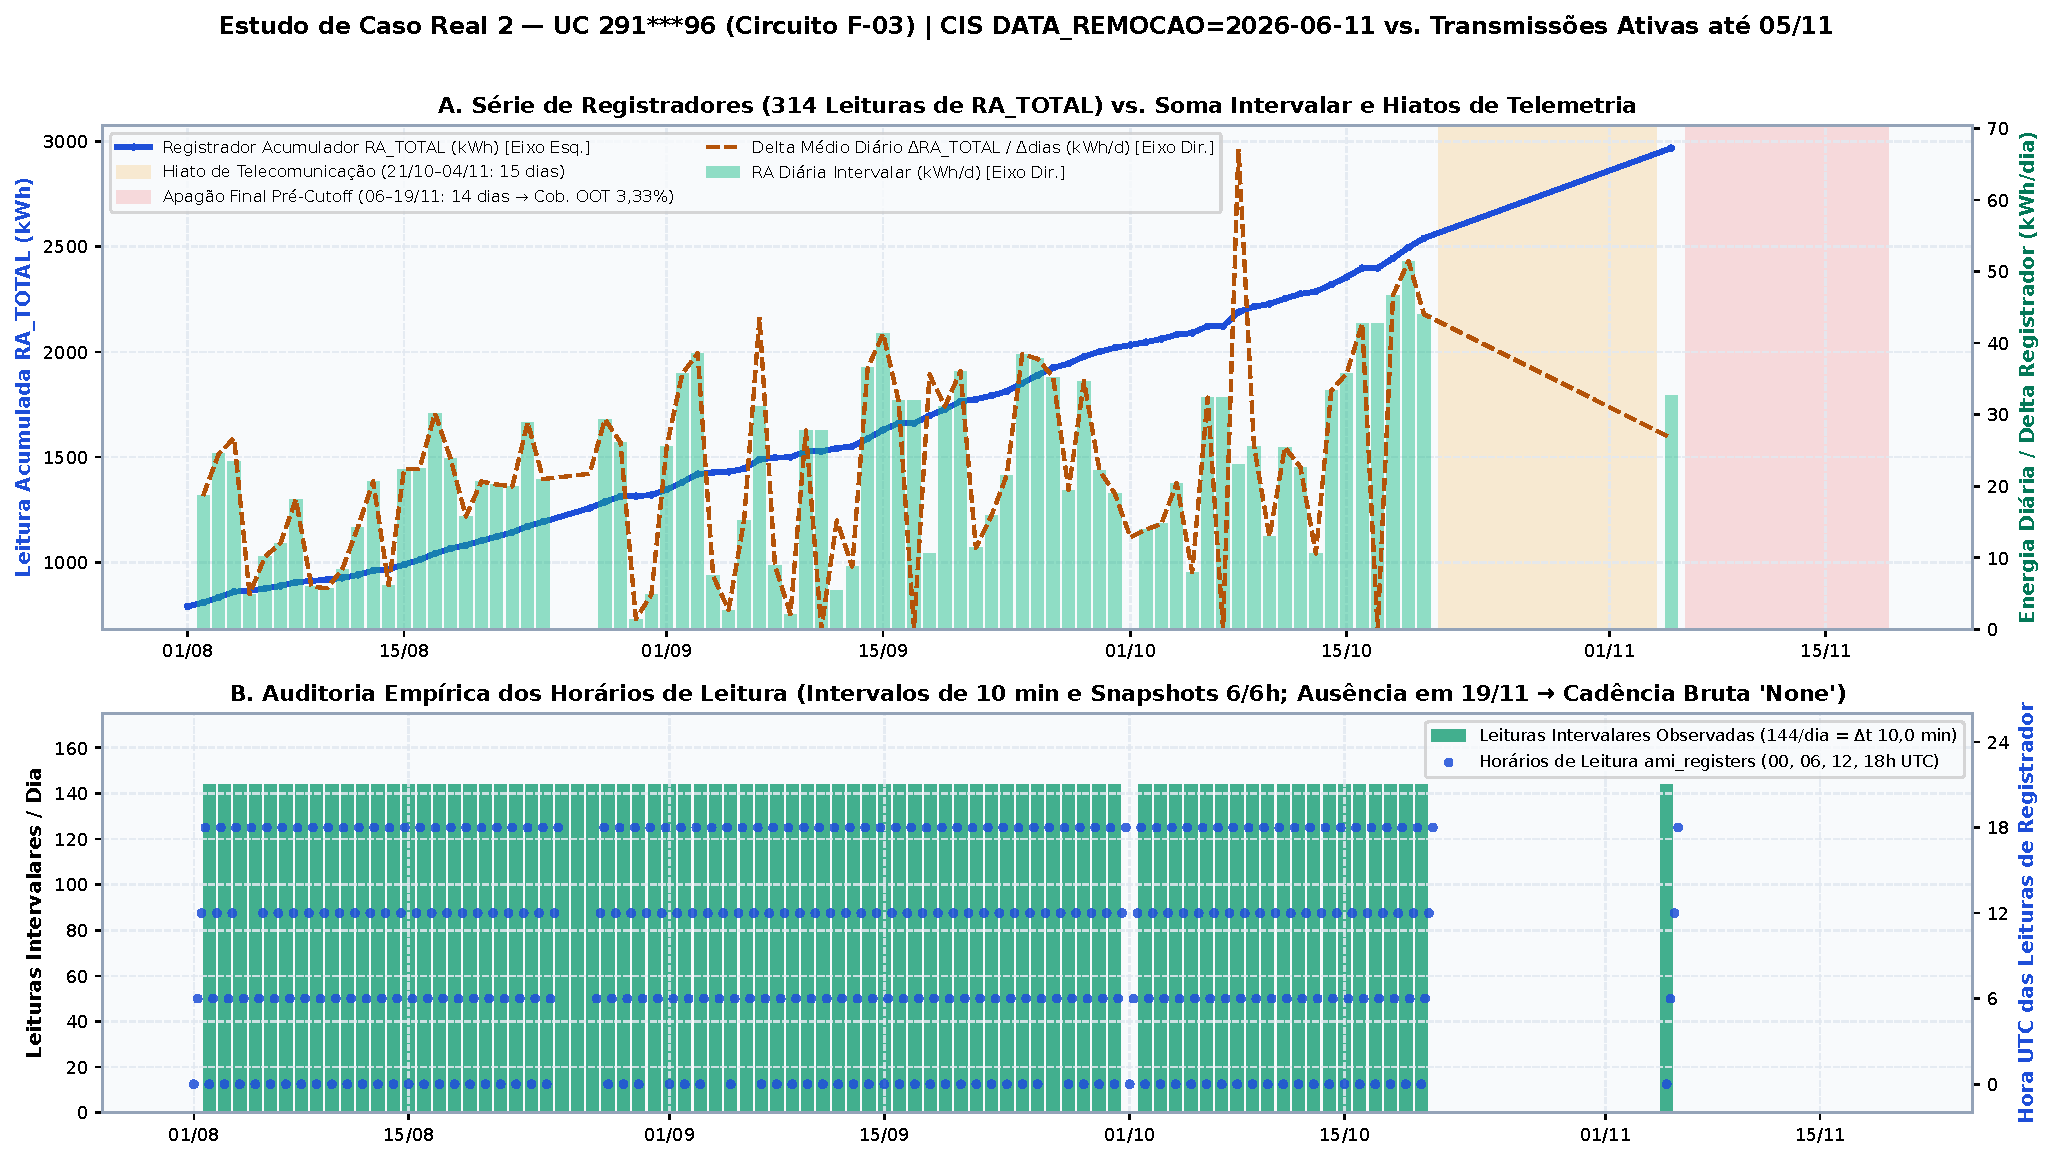
\includegraphics[width=0.96\textwidth,height=0.46\textheight,keepaspectratio]{figuras/fig_caso_291xxx96_horarios_registradores.pdf}
\par\small Fonte: elaboração própria a partir de \texttt{ami\_interval} e \texttt{ami\_registers}.
\end{figure}

Na UC \texttt{685***20} (\texttt{NIO-437***86}), a divergência entre a apuração horária em grade fixa de 168 horas (29/10 a 04/11/2026) e a janela analítica de 30 dias foi fechada nos dados de origem (Figura \ref{fig:caso-685xxx20-reconciliacao} e Tabela \ref{tab:reconciliacao-uc-685xxx20}). O medidor operou em cadência nativa de 10 minutos (6 leituras/h; 144 intervalos/dia): ao dividir 6 leituras observadas pelos 12 slots de uma grade fixa de 5 minutos, obtinha-se 50,00\% constante; no denominador nativo de 10 minutos ($6/6$), a cobertura horária nas 168 horas foi de 100,00\%. Na janela de 30 dias em \texttt{uc\_day\_features} (06/10 a 04/11/2026), registraram-se 4.298 intervalos de 4.320 esperados ($30 \times 144$), resultando em 99,49\% de cobertura. No corte OOT de 19/11/2026 (\texttt{20261125\_134559\_972\_oot\_multiview}), a execução OOT reportou 30 dias confiáveis, cobertura de 99,49\% e escore elétrico consolidado de 0,9850. A apuração de 4.298/4.320 apresentada na figura refere-se especificamente à janela de 06/10 a 04/11, não à janela de 30 dias terminada em 19/11.

\begin{figure}[htbp]\centering\caption{Reconciliação da cobertura da UC \texttt{685***20} (\texttt{NIO-437***86}, cadência nativa $\Delta t = 10$~min): (A) série horária observada (168h entre 29/10 e 04/11/2026); (B) cobertura horária em grade fixa de 5~min ($6/12 = 50{,}0\%$) versus cadência nativa de 10~min ($6/6 = 100{,}0\%$); (C) janela de 30 dias em \texttt{uc\_day\_features} ($4.298 / 4.320 = 99{,}49\%$)}\label{fig:caso-685xxx20-reconciliacao}
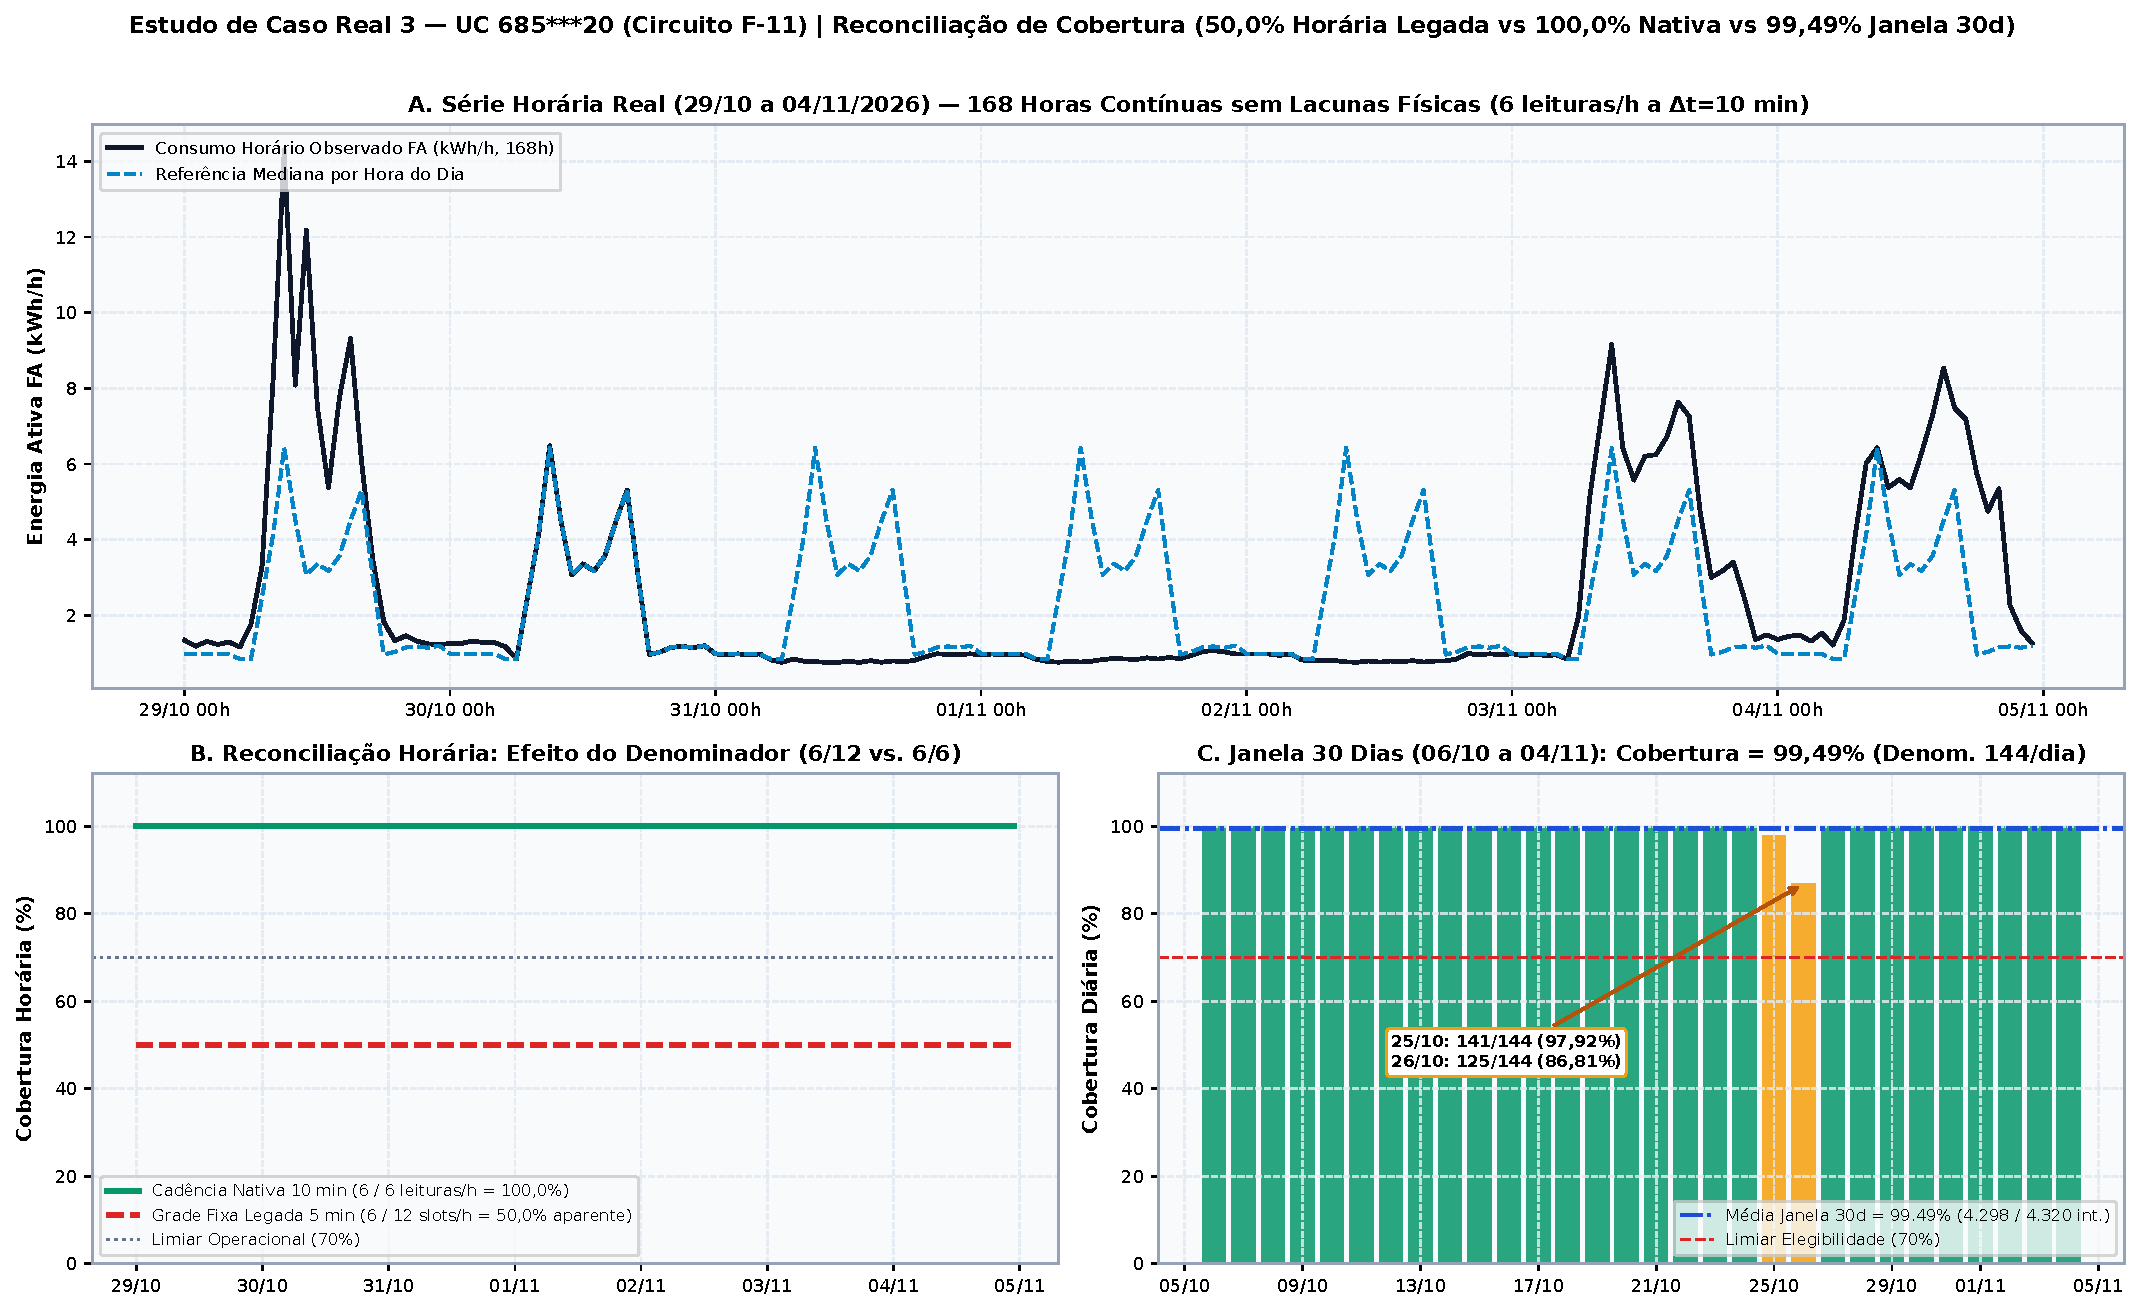
\includegraphics[width=0.96\textwidth,height=0.46\textheight,keepaspectratio]{figuras/fig_caso_685xxx20_reconciliacao_cobertura.pdf}
\par\small Fonte: elaboração própria a partir de \texttt{ami\_interval} e \texttt{uc\_day\_features}.
\end{figure}

\begin{table}[htbp]\centering\small\caption{Reconciliação formal entre representações de cobertura observadas para a UC \texttt{685***20} (\texttt{NIO-437***86}) sem alteração de valores originais}\label{tab:reconciliacao-uc-685xxx20}
\setlength{\tabcolsep}{3pt}
\begin{tabular}{@{}>{\raggedright\arraybackslash}p{0.20\linewidth}>{\raggedright\arraybackslash}p{0.20\linewidth}>{\raggedright\arraybackslash}p{0.22\linewidth}>{\raggedright\arraybackslash}p{0.17\linewidth}>{\raggedleft\arraybackslash}p{0.11\linewidth}@{}}\toprule
Representação & Canal/cadência & Período & Observado / esperado & Valor \\ \midrule
Horária legada & \texttt{ami\_interval.FA}, 10~min & 168~h\newline\mbox{29/10--04/11} & 6/12 por hora (5~min) & 50,00\% \\
Horária nativa & \texttt{ami\_interval.FA}, 10~min & 168~h\newline\mbox{29/10--04/11} & 6/6 por hora (10~min) & 100,00\% \\
Janela 30 dias & \texttt{uc\_day\_}\allowbreak\texttt{features}, 10~min & 30 dias\newline\mbox{06/10--04/11} & 4.298/4.320 & 99,49\% \\
Instantânea diária (grade legada) & \texttt{ami\_}\allowbreak\texttt{instantaneous}, 20~min & Diário (30 dias) & 72/288 por dia & 25,00\% \\
\bottomrule\end{tabular}
\par\small Fonte: elaboração própria a partir dos registros de origem.
\end{table}
